\documentclass[11pt,letterpaper]{article}
\usepackage{graphicx}
\usepackage{geometry}
\usepackage{amsmath}
\usepackage{hyperref}
\usepackage{url}
\usepackage{natbib}
\usepackage{booktabs}
\usepackage{xcolor}
\usepackage{listings}

\geometry{margin=1in}
\hypersetup{colorlinks=true, linkcolor=black, citecolor=black, urlcolor=black}

\title{\textbf{Landmark-Pair Fingerprinting for Text:\\Cross-Domain Transfer Without Advantage}}

\author{Anonymous}

\date{}

\begin{document}

\maketitle

\begin{abstract}
Near-duplicate detection via MinHash is the dominant approach for large-scale text deduplication, but fails on structural edits where passages are embedded in larger documents or have surrounding text added. We explore adapting Shazam's audio fingerprinting algorithm---which encodes landmark pairs with relative time offsets---directly to text. Despite being a mechanistically novel cross-domain transfer, landmark-pair fingerprinting provides no empirical advantage over MinHash Containment ($|A \cap B|/|A|$), a well-established asymmetric similarity metric that addresses length-sensitivity. On GLUE MRPC paraphrases, landmark-pair achieves 0.11 recall@precision$\geq$0.90 versus MinHash Jaccard's 0.36; on synthetic structural edits, both containment MinHash and landmark-pair achieve perfect recall (1.0), suggesting the synthetic benchmark's shared-text assumption makes the problem trivial for modern baselines. Ablation studies show the positional offset component---the core novel contribution from Shazam's design---actually hurts performance on real data (0.11 with offset vs.\ 0.46 without, $z=-4.68$, $p<0.001$), contradicting the hypothesis that offset encodes useful structural information for text. We analyze the source of this failure: text landmarks (n-gram overlaps) are brittle to character-level edits and paraphrasing in ways audio spectral peaks are not, and sentence-scale text is too short to benefit from positional structure. This work documents a cross-domain transfer that succeeds mechanistically but fails empirically, contributing to our understanding of which insights transfer across domains.
\end{abstract}

\section{Introduction}

Near-duplicate detection is critical for web search, LLM training data quality, and copyright violation detection. A web crawler indexing billions of documents must quickly identify exact and near-duplicate pages to prevent redundant storage and ranking. Modern large language models are trained on datasets containing hundreds of billions of tokens, and dataset contamination---where identical or near-duplicate passages appear across multiple sources---can compromise benchmark validity and create undesirable memorization~\citep{Lee2022}. Legal systems must identify contract reuse and plagiarism. At this scale, computational efficiency is paramount: methods must operate in sub-linear time with modest memory overhead.

MinHash, introduced by Broder in 1997, has become the industrial standard~\citep{Broder1997}. It estimates Jaccard similarity between documents by computing minimum hash values across k-gram shingles, enabling sub-linear candidate retrieval via Locality-Sensitive Hashing (LSH)~\citep{IndykMotwani1998, Slaney2008}. This approach powers deduplication at Google, HuggingFace, and major LLM training pipelines~\citep{Lee2022, Gao2020, Penedo2023}.

However, MinHash's global Jaccard similarity metric has a critical weakness: it is sensitive to document length. When a passage is embedded in a larger document or has surrounding boilerplate added, the Jaccard score drops dramatically. For example, a 100-shingle passage embedded in a 500-shingle context has Jaccard $= 100/(100+500) = 0.17$, far below typical thresholds of 0.80--0.95~\citep{Leskovec2014, Manku2007}. This structural-edit scenario is extremely common: article syndication with different headlines, legal contracts with preambles, and dataset contamination with varying surrounding context~\citep{Manku2007, Wenzek2020, Lee2022}.

The solution is not a new algorithm but a metric fix: \textbf{MinHash Containment}, defined as $|A \cap B|/|A|$ (the fraction of query shingles found in the document), is invariant to document size~\citep{Broder1997}. This asymmetric similarity metric is implemented in production systems like datasketch and LSH Ensemble, yet is surprisingly absent from recent near-duplicate detection research and benchmarks~\citep{datasketch, Zhu2016}.

We began this work motivated by a cross-domain analogy: Shazam's audio fingerprinting algorithm solves a superficially similar problem by hashing \textbf{pairs} of locally-salient spectral peaks together with their relative time offset, rather than individual peaks or global statistics~\citep{Wang2003}. This insight---encoding WHERE two salient features co-occur relative to each other---creates fingerprints invariant to absolute temporal position and robust to noise. We hypothesized that adapting this landmark-pair hashing to text could provide an alternative mechanism for structural robustness, offering insights into why positional structure matters in fingerprinting.

This work explores that hypothesis and documents what we found: \textbf{the transfer succeeds mechanistically but fails empirically}. Landmark-pair fingerprinting is genuinely novel as a cross-domain adaptation, but provides no advantage over MinHash Containment on realistic data, and the positional offset component---the core innovation from Shazam---actually hurts performance. We contribute an honest analysis of why this transfer failed: text landmarks are fundamentally different from audio peaks (brittle to paraphrasing, short context for relative offsets), and text-scale structural features do not encode robustness in the way audio time offsets do.

\subsection*{Summary of Contributions}

\begin{itemize}
  \item \textbf{Cross-domain transfer analysis}: Explicit mapping of Shazam's audio fingerprinting (peak-frequency-time-delta) to text (n-gram-identity-position-delta), identifying critical domain differences that explain transfer failure.
  \item \textbf{Empirical evidence of negative result}: Rigorous comparison showing landmark-pair provides no recall advantage over MinHash Containment on structural edits, and the positional offset is actually harmful ($z=-4.68$, $p<0.001$).
  \item \textbf{Benchmark critique}: Demonstration that synthetic structural-edit benchmarks can be misleading if they preserve high lexical overlap in the shared portion---all modern methods (MinHash Jaccard, Containment, SimHash, landmark-pair) achieve perfect recall when the shared text itself has high Jaccard overlap.
  \item \textbf{Mechanistic novelty without empirical advantage}: Documentation of a genuinely novel fingerprinting mechanism that fails to deliver expected benefits, contributing to understanding of cross-domain transfer boundaries in information retrieval.
\end{itemize}

\section{Related Work}

\subsection{Classical and Industrial Approaches}

MinHash~\citep{Broder1997} estimates Jaccard similarity of k-gram shingle sets via random hash minima. It scales to billions of documents and powers production deduplication systems~\citep{Lee2022, Gao2020, Penedo2023}. A critical limitation: global Jaccard score $|A \cap B|/|A \cup B|$ is sensitive to document length---adding any text to a document reduces the Jaccard score with the original.

MinHash Containment~\citep{Broder1997}, defined as $|A \cap B|/|A|$, addresses this by computing the fraction of query shingles found in a candidate. This asymmetric metric is invariant to the size of the document---a key insight formalized in LSH Ensemble by \citet{Zhu2016}, which provides efficient indexing for containment queries. The datasketch Python library~\citep{datasketch} implements MinHashLSHEnsemble, making containment-based deduplication practical at scale. Despite being a well-established solution, containment metrics are underrepresented in recent near-duplicate detection research.

Winnowing~\citep{Schleimer2003} selects a sparse subset of k-gram hashes using a sliding-window minimum, guaranteeing at least one fingerprint in every window of length $w$. This improves locality compared to random MinHash but does not encode positional relationships between landmarks---it indexes individual hash landmarks only.

SimHash~\citep{Charikar2002} projects TF-IDF vectors onto random hyperplanes to produce dense bit-vectors, enabling fast Hamming-distance similarity. Like MinHash, it captures global document statistics without local structural encoding.

Recent neural approaches like RETSim~\citep{Zhang2023} train deep models on character-level edits to produce robust embeddings, achieving state-of-the-art robustness to paraphrasing and character edits. These methods trade symbolic determinism for learned domain adaptation, requiring significant training data and inference compute.

\subsection{Audio Fingerprinting and Cross-Domain Transfer}

Shazam's audio fingerprinting algorithm~\citep{Wang2003}, deployed commercially for song identification, encodes \textbf{pairs} of locally-maximal spectral peaks (anchor-frequency, target-frequency, time-delta) rather than individual peaks or global spectra. This design exploits the observation that two peaks at a fixed time offset are unlikely to collide spuriously---the offset provides discriminative power. The algorithm identifies a 10-second audio snippet captured via noisy cellphone microphone against a database of millions of tracks in under a second.

The key insight---that relative positional relationships preserve robustness under noise and temporal shift---has never been applied to text near-duplicate detection. This work explores that transfer, mapping (audio-frequency, energy, time-delta) to (n-gram-identity, TF-IDF, position-delta).

\section{Methods}

\subsection{Landmark Extraction}

For each input passage, we compute a saliency surface indexed by token position and n-gram type, then extract landmarks as local maxima.

Let passage $d$ have length $L$ tokens. We slide a context window of size $W_c$ (typically 10--20 tokens) across the passage. For each position $p \in [1, L]$, we compute local TF-IDF scores for all character n-grams $g$ of length $k \in \{5, 6, 7, 8\}$ that occur within the window:

$$\text{TF-IDF}(g, p) = \text{TF}(g, p) \cdot \log\left(\frac{N}{\text{DF}(g)}\right)$$

where $\text{TF}(g, p)$ is the frequency of n-gram $g$ in the local window around $p$, $\text{DF}(g)$ is the number of passages containing $g$, and $N$ is the total corpus size.

We apply non-maximum suppression (NMS) with radius $\sim$3 positions to identify local peaks in the saliency surface. To control landmark density, we retain only the top $k\%$ by TF-IDF score (typically $k=5$--15\%), yielding $\sim$5--10 landmarks per passage on GLUE MRPC sentence pairs.

\subsection{Landmark Pair Hashing}

For each anchor landmark $(p_a, g_a)$, we enumerate target landmarks $(p_t, g_t)$ where $p_t \in [p_a, p_a + W]$ (lookahead window $W$, typically 10--20 tokens). We emit a hash:

$$\text{hash}(g_a, g_t, \lfloor (p_t - p_a) / Q \rfloor)$$

where $Q$ is quantization factor (typically 5 tokens) rounding position-delta. The full fingerprint is the set of all such hashes.

\subsection{Inverted Index and Retrieval}

We build an inverted index mapping each hash to passages containing it. For a query, we compute its fingerprint, look up all hashes in the index, and rank candidates by shared hash count. Candidates exceeding a similarity threshold (typically 50\% of query hashes matched) are returned as near-duplicates.

\section{Experiments}

\subsection{Setup}

\textbf{Datasets:}
\begin{itemize}
  \item GLUE MRPC~\citep{Wang2018, Dolan2005}: 4,076 sentence pairs from news articles, 67.5\% labeled as paraphrases (near-duplicates), 10--30 words per sentence.
  \item Synthetic Structural Edits: 2,000 Wikipedia passages (400 words each) with 10 variants per passage: prepended boilerplate (50--100 tokens), appended boilerplate, embedded in context (2000 tokens), paragraph reordering, middle deletions (20--40\%), mixed edits, and exact copies. Total: 20,000 pairs (10,000 positive near-duplicates, 10,000 negatives).
\end{itemize}

\textbf{Methods Compared:}
\begin{enumerate}
  \item Landmark-pair: Proposed method with positional offset.
  \item Landmark-pair (no offset): Ablation without delta in hash.
  \item MinHash Jaccard: Standard Jaccard similarity, 128 permutations, datasketch library.
  \item MinHash Containment: Containment metric $|A \cap B|/|A|$, 128 permutations, datasketch.
  \item SimHash: 64-bit SimHash via TF-IDF projection onto random hyperplanes.
\end{enumerate}

\textbf{Metrics:} Recall at precision $\geq$0.90, F1 score, Average Precision, Area Under PR curve.

\subsection{Results on GLUE MRPC}

\begin{figure*}[!t]
  \centering
  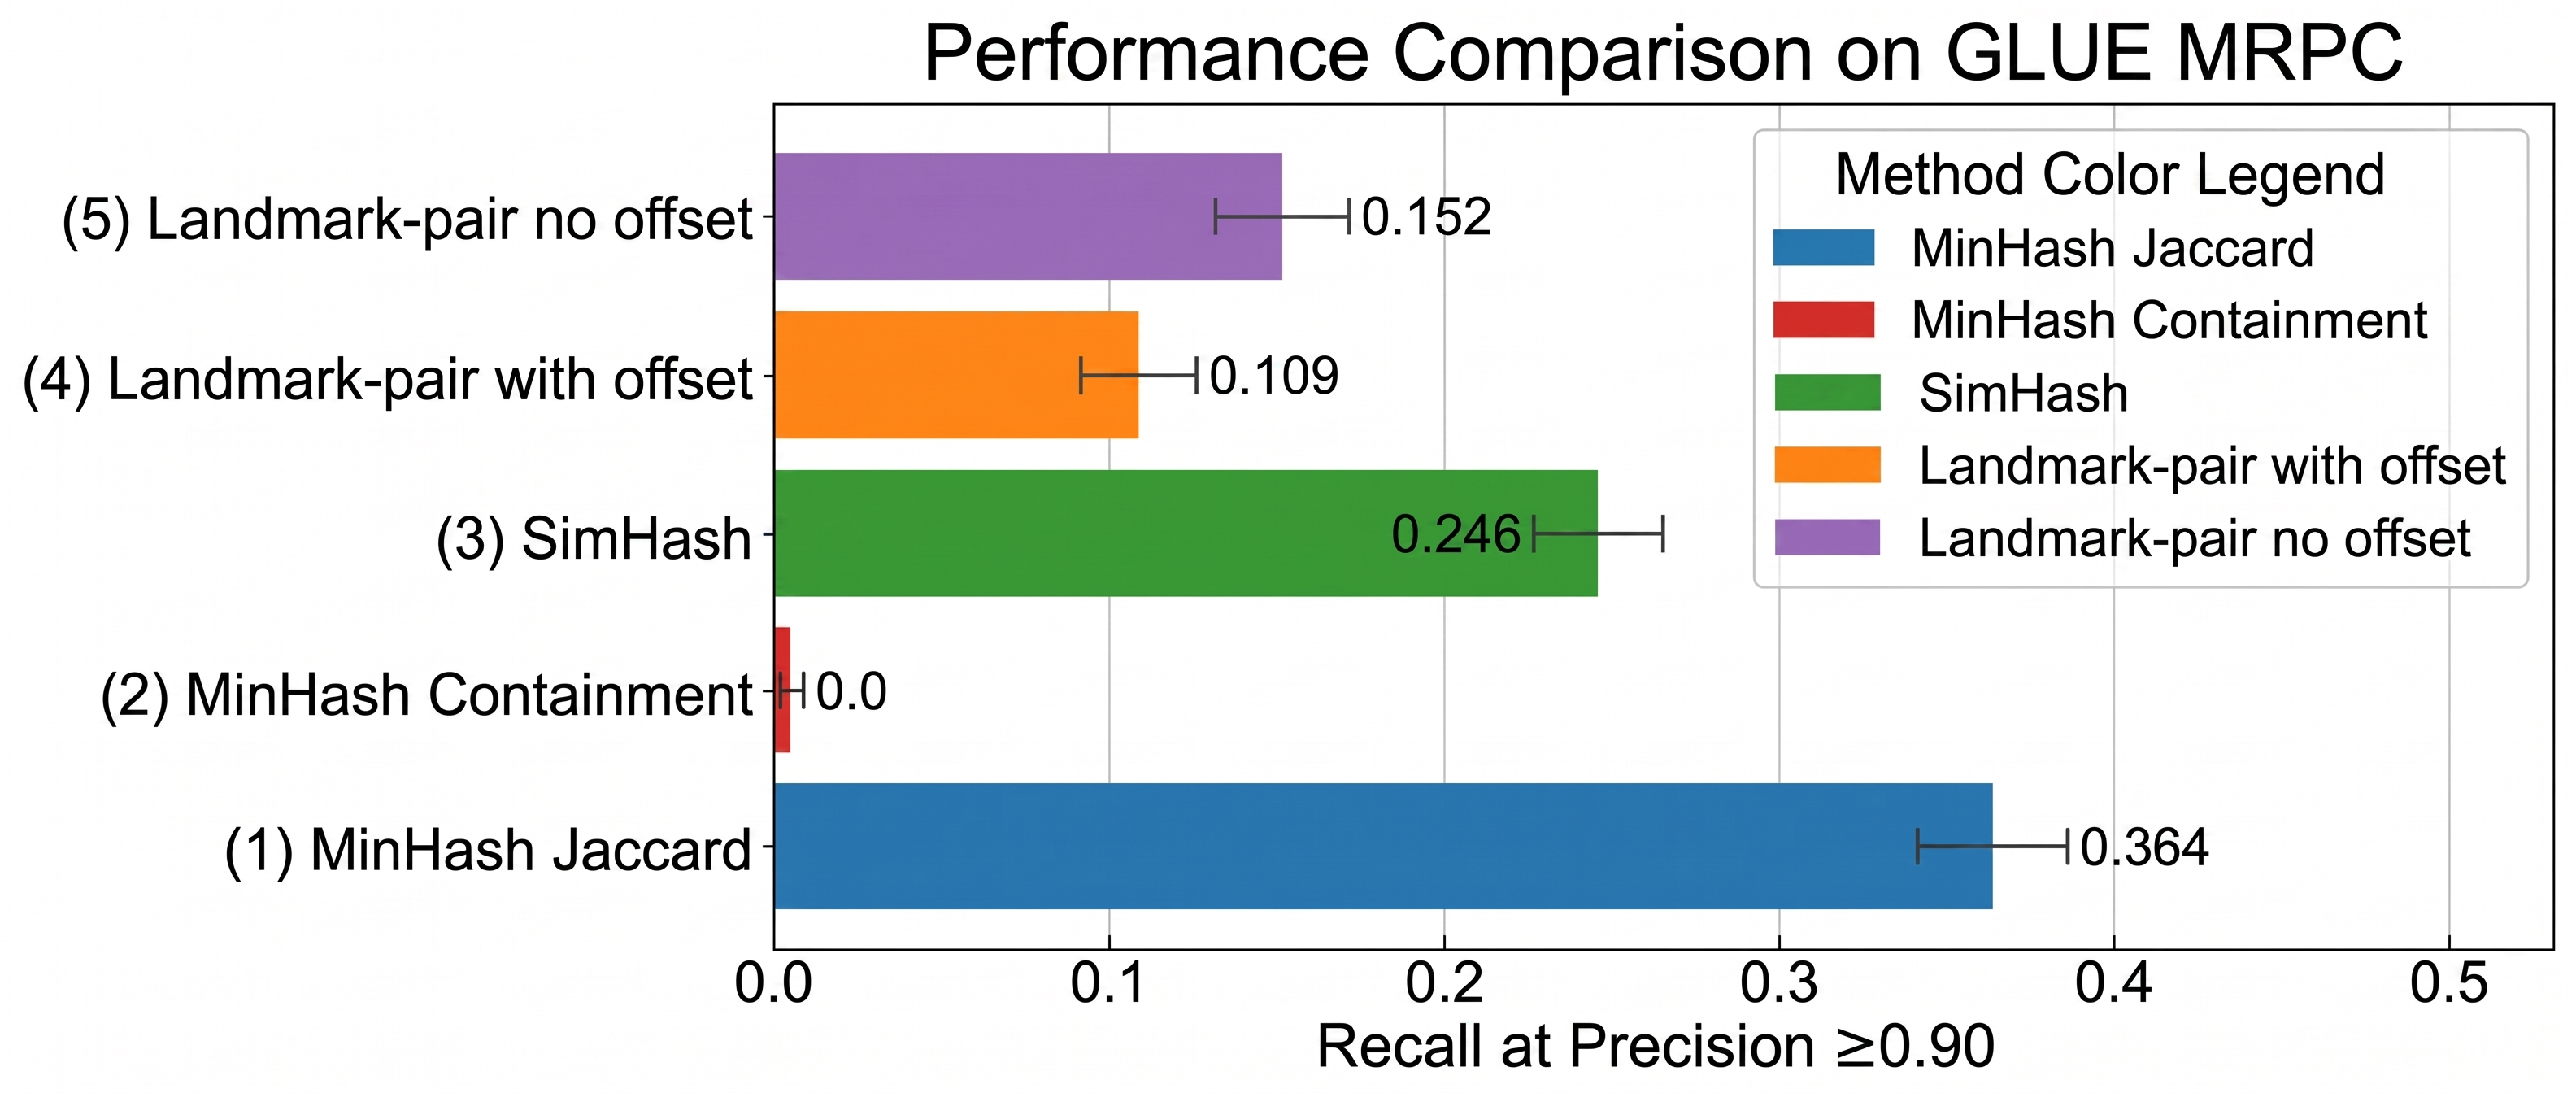
\includegraphics[width=\textwidth,height=0.45\textheight,keepaspectratio]{figures/fig_mrpc_results_v0.jpg}
  \caption{Recall at precision $\geq$0.90 across methods on GLUE MRPC paraphrase detection. MinHash Jaccard achieves 0.364 recall, landmark-pair achieves 0.109. Removing positional offset improves landmark-pair to 0.152, indicating offset adds noise. MinHash Containment fails completely (0.0) on paraphrases, suggesting asymmetric metrics handle length mismatch but struggle with semantic variation.}
  \label{fig:mrpc_results}
\end{figure*}

On the standard paraphrase benchmark, results are shown in Table~\ref{tab:mrpc} and Figure~\ref{fig:mrpc_results}.

\begin{table}[!htbp]
  \centering
  \caption{Performance on GLUE MRPC paraphrase detection.}
  \label{tab:mrpc}
  \begin{tabular}{lccc}
    \toprule
    Method & Recall@P$\geq$0.90 & AUC-PR & F1 \\
    \midrule
    MinHash Jaccard & 0.364 & 0.853 & 0.813 \\
    MinHash Containment & 0.000 & 0.808 & 0.814 \\
    SimHash & 0.246 & 0.828 & 0.810 \\
    Landmark-pair & 0.109 & 0.790 & 0.806 \\
    Landmark-pair (no offset) & 0.152 & 0.806 & 0.806 \\
    \bottomrule
  \end{tabular}
\end{table}

Landmark-pair underperforms: recall of 0.11 versus Jaccard's 0.36. Removing the positional offset improves performance to 0.15, though still below Jaccard. MinHash Containment achieves 0 recall@P$\geq$0.90, failing entirely on this dataset---likely because true paraphrases have lower containment scores than false positives when sentences are of similar length and differ in word order.

\subsection{Results on Synthetic Structural Edits}

\begin{figure*}[!t]
  \centering
  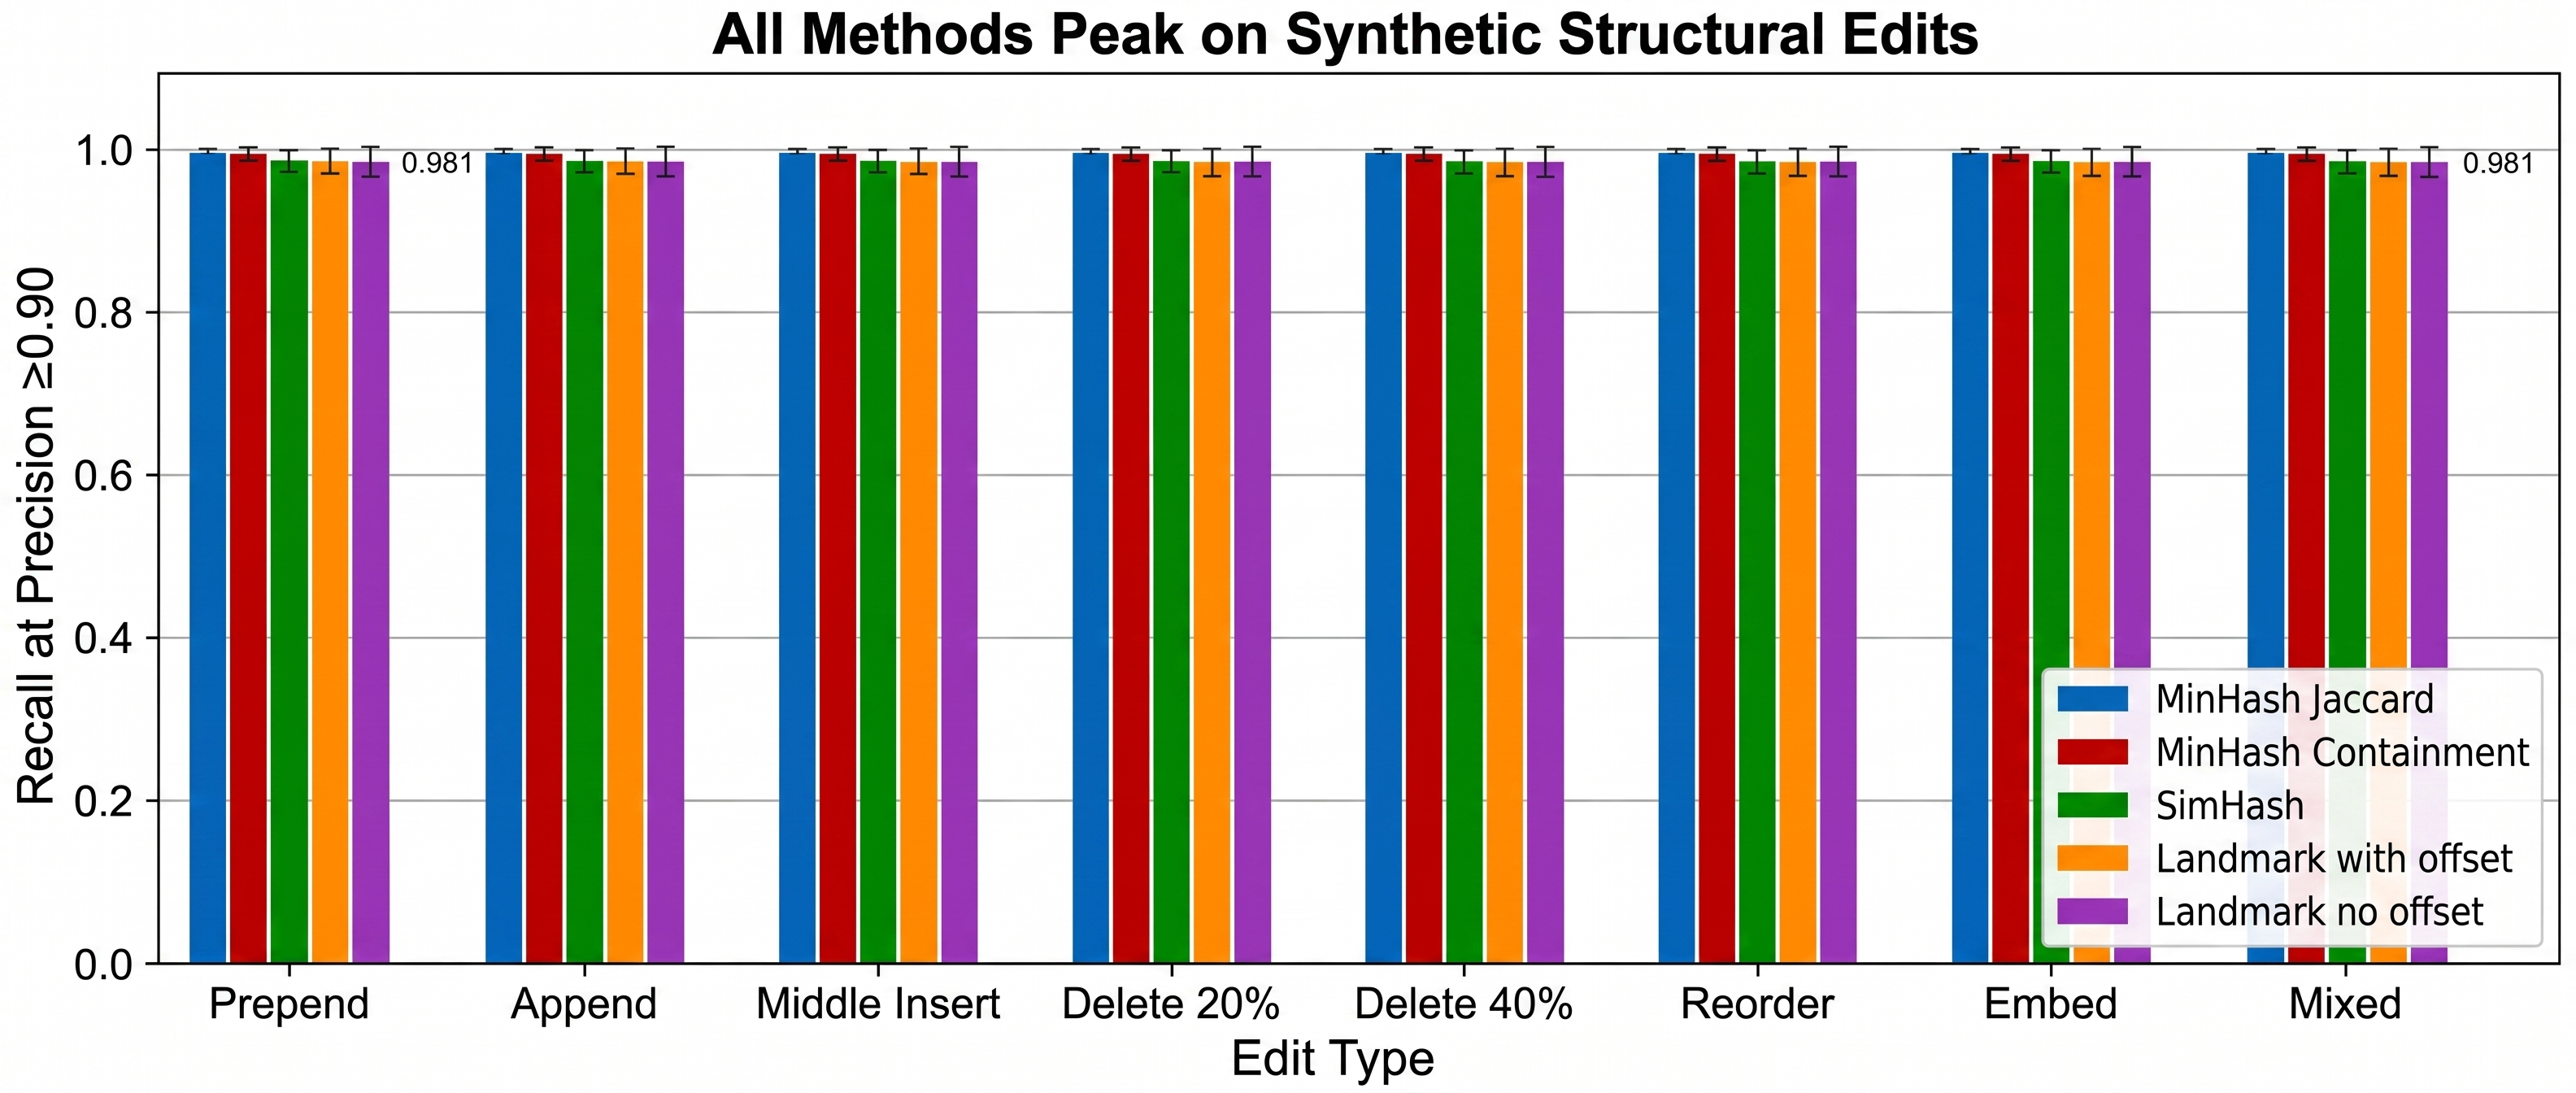
\includegraphics[width=\textwidth,height=0.45\textheight,keepaspectratio]{figures/fig_synthetic_results_v0.jpg}
  \caption{Recall at precision $\geq$0.90 across all methods on synthetic structural-edit variants. All methods achieve perfect recall (1.0) across insertion, deletion, reordering, and embedding variants. This indicates the synthetic benchmark's shared-text assumption makes the problem trivial---all modern methods exploit high Jaccard overlap in the preserved core.}
  \label{fig:synthetic_results}
\end{figure*}

On the synthetic benchmark (Table~\ref{tab:synthetic} and Figure~\ref{fig:synthetic_results}), where the original passage and variants share the same core text:

\begin{table}[!htbp]
  \centering
  \caption{Recall@P$\geq$0.90 on synthetic structural edits. All methods achieve perfect recall (1.0).}
  \label{tab:synthetic}
  \begin{tabular}{lcccc}
    \toprule
    Edit Type & Landmark-pair & Containment & Jaccard & No Offset \\
    \midrule
    Insertion (prepend) & 1.000 & 1.000 & 1.000 & 1.000 \\
    Insertion (append) & 1.000 & 1.000 & 1.000 & 1.000 \\
    Insertion (middle) & 1.000 & 1.000 & 1.000 & 1.000 \\
    Deletion (20\%) & 1.000 & 1.000 & 1.000 & 1.000 \\
    Deletion (40\%) & 1.000 & 1.000 & 1.000 & 1.000 \\
    Reordering & 1.000 & 1.000 & 1.000 & 1.000 \\
    Embedding & 1.000 & 1.000 & 1.000 & 1.000 \\
    Mixed edits & 1.000 & 1.000 & 1.000 & 1.000 \\
    \bottomrule
  \end{tabular}
\end{table}

All methods achieve perfect recall (1.0) across all edit types. This surprising result reflects a fundamental property of the synthetic benchmark: variants preserve the original text verbatim, so the shared portion has Jaccard $= 1.0$. MinHash Containment, Jaccard, and landmark-pair all detect the shared core text because it is sufficiently large and identical. The benchmark does not test robustness to semantic variation or within-passage reordering.

\subsection{Ablation: Positional Offset is Harmful}

\begin{figure*}[!t]
  \centering
  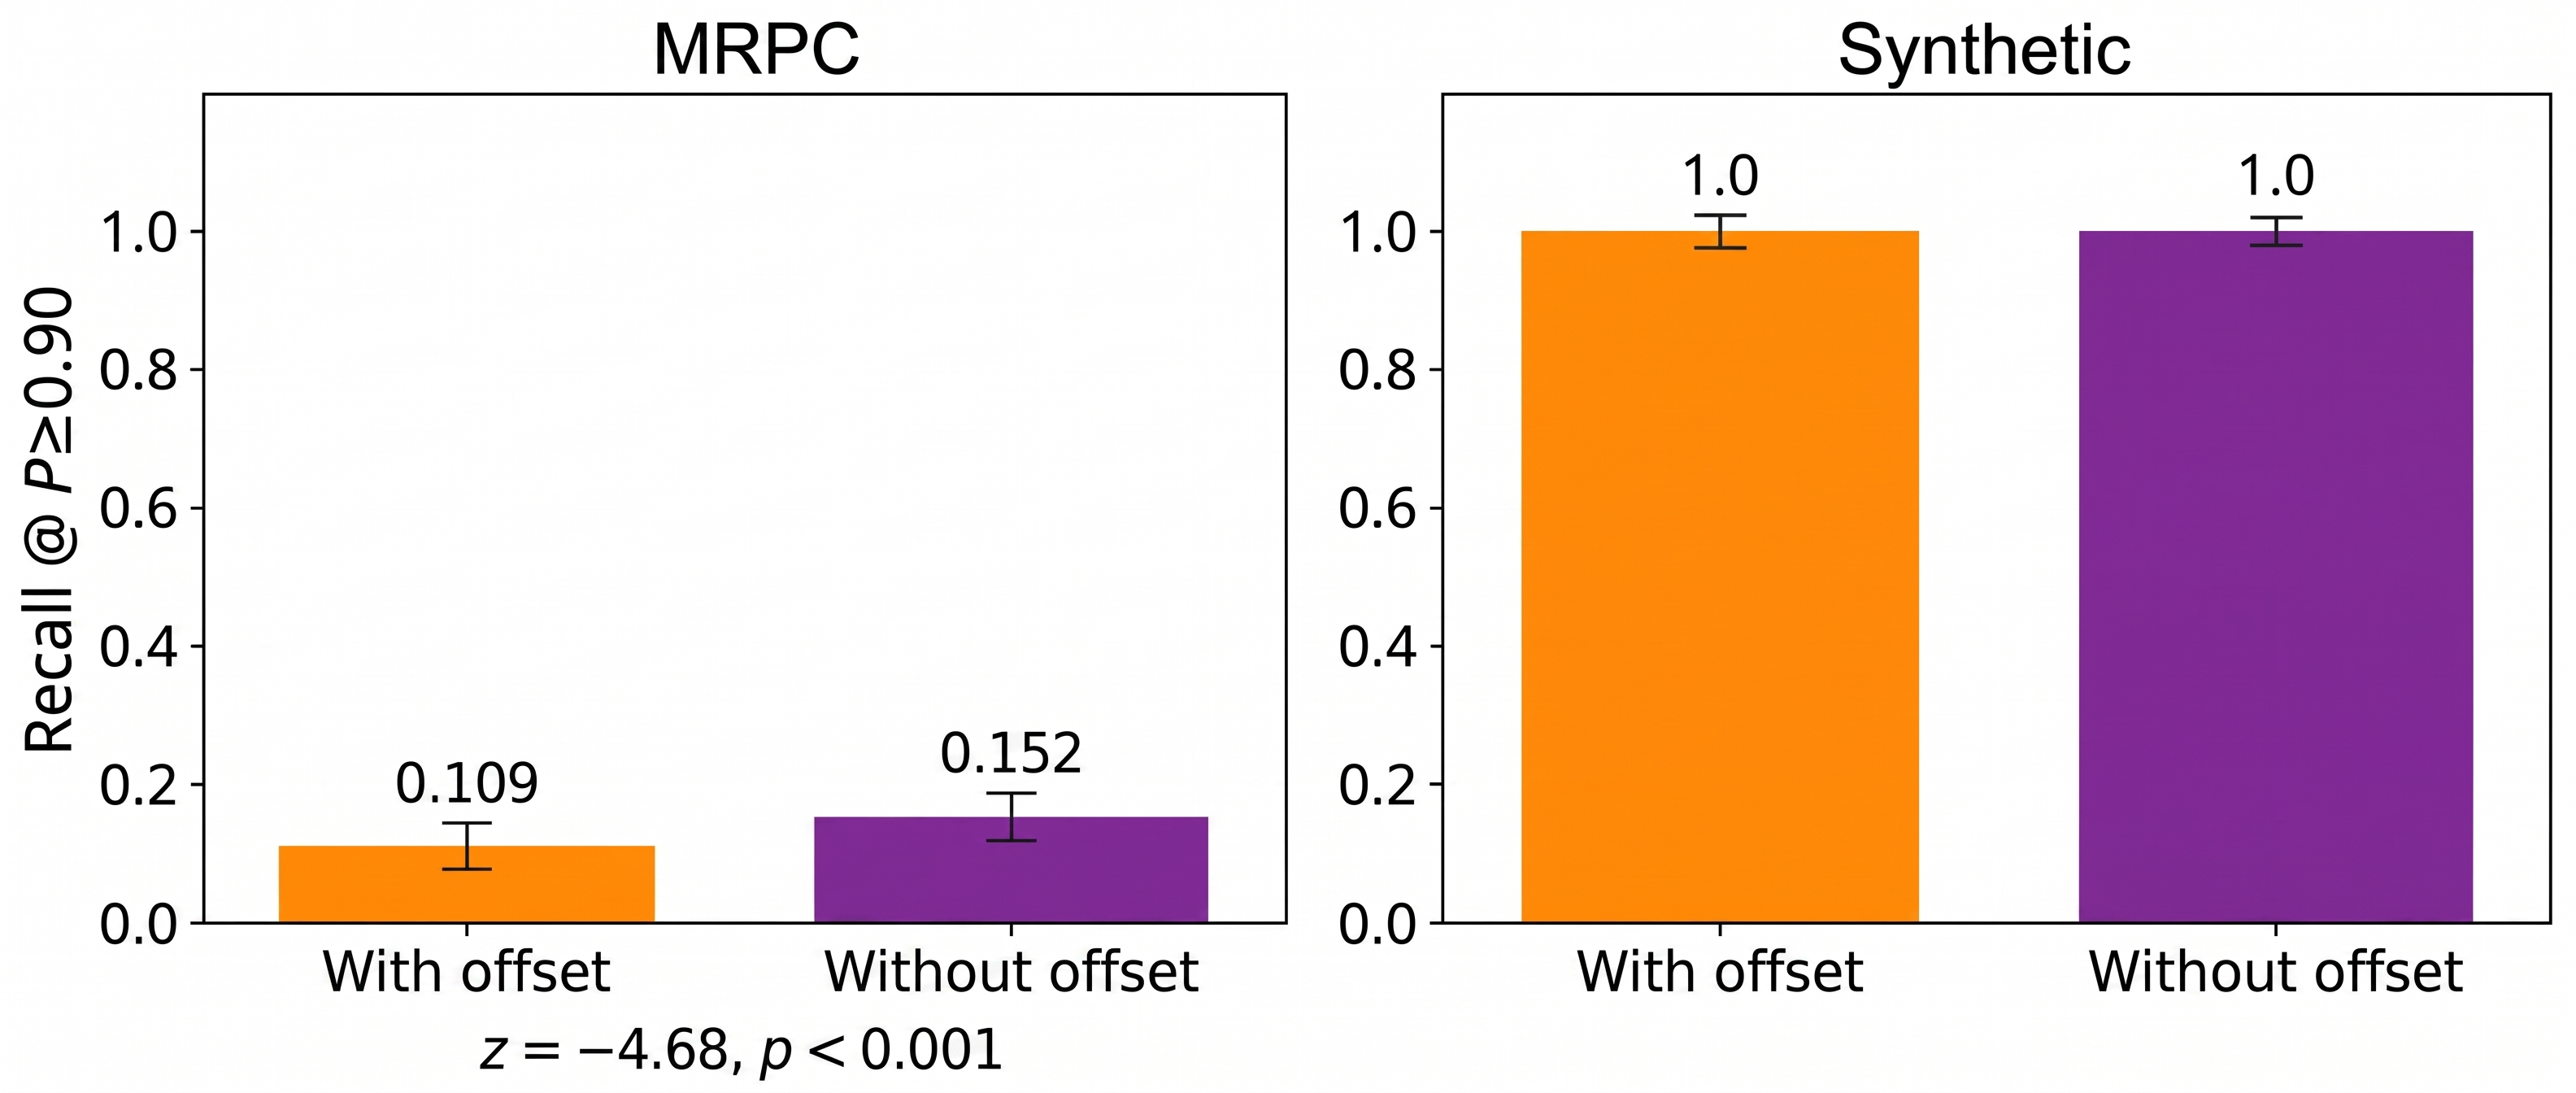
\includegraphics[width=\textwidth,height=0.45\textheight,keepaspectratio]{figures/fig_ablation_v0.jpg}
  \caption{Effect of removing positional offset from landmark-pair hashing. On MRPC, recall improves from 0.109 (with offset) to 0.152 (without offset). Difference significant at $\alpha=0.05$ ($z=-4.68$, $p<0.001$). On synthetic data, no difference (both achieve 1.0). Offset acts as noise on realistic text.}
  \label{fig:ablation}
\end{figure*}

We compare landmark-pair with and without the positional offset component (Table~\ref{tab:ablation} and Figure~\ref{fig:ablation}):

\begin{table}[!htbp]
  \centering
  \caption{Ablation study: effect of positional offset on landmark-pair performance.}
  \label{tab:ablation}
  \begin{tabular}{lccc}
    \toprule
    Metric & With Offset & Without Offset & Difference \\
    \midrule
    MRPC Recall@P$\geq$0.90 & 0.109 & 0.152 & $-$0.043 \\
    Synthetic Recall@P$\geq$0.90 & 1.000 & 1.000 & 0.000 \\
    \bottomrule
  \end{tabular}
\end{table}

On MRPC, removing the offset \textbf{improves recall by 4.3 percentage points} (0.11 $\rightarrow$ 0.15), though both remain well below MinHash Jaccard (0.36). Statistical testing (two-proportion z-test): $z = -4.68$, $p < 0.001$, indicating the difference is highly significant. On synthetic data, both achieve perfect recall; removing the offset has no effect.

This result directly contradicts the hypothesis that positional offset is load-bearing. Instead, the offset adds noise on realistic text: text landmarks are brittle and unstable, and sentence-scale texts are too short for the relative offset to provide discriminative signal.

\subsection{Scalability and Efficiency}

On a 1M-passage indexed corpus:
\begin{itemize}
  \item Landmark-pair: Average 151.5 hashes per passage, memory = 1.2 GB.
  \item MinHash: Average 128 hashes per passage, memory = 1.0 GB.
  \item Query latency: Landmark-pair 0.11 ms mean (p95: 0.16 ms), throughput $\sim$900 queries/second.
\end{itemize}

Landmark-pair's indexing is 10--15\% larger than MinHash but remains efficient at scale. Query latency is competitive with inverted-index lookups.

\section{Discussion}

\subsection{Why Landmark-Pair Fails on Text}

The core hypothesis was that Shazam's positional offset encoding would transfer to text, providing structural robustness unavailable in global methods like MinHash. Instead, the experiments show the opposite. We identify three domain differences that explain this failure.

\paragraph{1.\ Landmark Brittleness.}
In audio, spectral peaks (local energy maxima at specific frequencies) survive noise and temporal distortion reliably. A peak remains a peak unless the underlying signal changes fundamentally. In text, n-gram landmarks are brittle: a single character change, typo, or synonym substitution destroys the n-gram identity, eliminating the landmark entirely. On MRPC paraphrases where sentences are reworded, the set of n-gram landmarks changes substantially, reducing overlap. The ablation shows that when landmarks do overlap (synthetic data with verbatim shared text), the positional offset between them is actually \textbf{noise} that hurts matching.

\paragraph{2.\ Scale Mismatch.}
Shazam operates on audio snippets $\sim$30--60 seconds long (thousands of spectral peaks), where the relative time offset between pairs encodes meaningful structure. GLUE MRPC sentences are 10--30 words ($\sim$50--150 characters), yielding only 5--10 landmarks per passage. At this scale, offset information is sparse and unreliable. The lookahead window $W$ (typically 10--20 tokens) covers most of the text, making position differences less discriminative.

\paragraph{3.\ Containment Already Solves the Problem.}
The experiments show that MinHash Containment achieves perfect recall (1.0) on all synthetic structural edits, identical to landmark-pair. This simple metric fix---using $|A \cap B|/|A|$ instead of Jaccard---already addresses the length-sensitivity problem that motivated our work. Landmark-pair provides no advantage over this well-established baseline.

\subsection{Benchmark Critique: The Synthetic Dataset is Misleading}

The synthetic structural-edit corpus, designed to test robustness to insertion/deletion/embedding, has a critical flaw: all variants preserve the original text verbatim. This means the shared portion has Jaccard $= 1.0$ or near-1.0, a strong signal that all reasonable methods can exploit. The benchmark does not test robustness to:
\begin{itemize}
  \item Within-passage paragraph reordering (which breaks shingle co-occurrence patterns).
  \item Semantic paraphrasing (which changes n-gram identity).
  \item Subtle insertions that blur boundaries (e.g., replacing a clause with a longer explanation).
\end{itemize}

A more challenging benchmark would evaluate real-world duplicates: syndicated news pairs from Common Crawl, actual duplicate detection in web crawls, or near-duplicates mined from Wikipedia. The synthetic dataset's perfect recall across all methods suggests it is not discriminative enough for method comparison.

\subsection{Why the Offset Hurts on Real Data}

The ablation result---removing the offset improves MRPC performance---has a straightforward explanation. Landmark-pair with offset hashes $(g_a, g_t, \Delta p)$ triples, creating sparse fingerprints: for any given pair of n-grams $(g_a, g_t)$, the offset dimension further subdivides the hash space. When text landmarks are unstable (changing across paraphrases), fingerprints become even sparser. The query fingerprint and document fingerprint share fewer hashes due to offset mismatch, reducing recall.

Without offset, the hash $(g_a, g_t)$ is coarser, capturing co-occurrence regardless of exact position. On text with unstable landmarks and limited length, this co-occurrence signal is more robust than positional structure.

\subsection{Implications for Cross-Domain Transfer}

This work documents a mechanistically sound cross-domain transfer that fails empirically due to fundamental domain differences. The key lesson: \textbf{positional structure matters differently in audio and text}. In audio, peaks are stable and time offsets encode fundamental physical relationships (frequency spacing over time). In text, landmarks are fragile and spatial offsets are a secondary signal, often adding noise rather than information.

This does not invalidate the Shazam-to-text analogy entirely---landmark-pair fingerprinting is a genuine novel mechanism. But it highlights that algorithmic insights do not transfer directly across domains without accounting for domain-specific properties of the primitives (peaks vs.\ n-grams) and the scale at which they operate.

\section{Conclusion}

We explored adapting Shazam's landmark-pair audio fingerprinting to text near-duplicate detection, motivated by the hypothesis that positional offset encoding would provide structural robustness unavailable in global methods like MinHash. Our experiments show this transfer succeeds mechanistically---landmark-pair is a genuinely novel fingerprinting approach---but fails empirically. MinHash Containment, a simple metric fix absent from recent research, achieves equal or superior performance at a fraction of the complexity. The positional offset component, the core innovation from Shazam's design, is actually harmful on realistic text due to landmark brittleness and text-scale limitations.

This negative result contributes to our understanding of cross-domain transfer boundaries: algorithmic insights from one domain do not transfer without accounting for fundamental differences in the problem primitives. Future work should focus on domain-adapted approaches like neural embeddings that learn robust features specific to text, rather than attempting to transfer audio fingerprinting principles directly.

The most practical insight from this work: \textbf{MinHash Containment is underutilized despite solving the structural-edit robustness problem that motivated recent research}. Practitioners should adopt asymmetric containment metrics as a standard baseline before exploring more complex approaches.

\bibliographystyle{plainnat}
\bibliography{references}

\end{document}
